%----------------------------------------------------------------------------------------
%	PACKAGES AND DOCUMENT CONFIGURATIONS
%----------------------------------------------------------------------------------------
\documentclass[11pt]{article}
\usepackage{amsmath} % Required for some math elements
\usepackage{hyperref} 
\usepackage{xcolor}
\usepackage{lipsum} 
\usepackage{cite}
\usepackage{graphicx} % Required for the inclusion of images
\usepackage{algorithmic}
\usepackage{array}
\usepackage{bookmark}
\usepackage{listings}
\usepackage{amssymb}
\usepackage{enumitem}
\usepackage[margin=24mm]{geometry}
\usepackage[caption=false, font=footnotesize]{subfig}
\usepackage{multirow}



\newlist{steps}{enumerate}{1}
\setlist[steps, 1]{label = Step \arabic*:}

\hypersetup{ %color attributes of citation, link, etc.
    colorlinks=true,
    linkcolor=blue,
    filecolor=gray,      
    urlcolor=blue,
    citecolor=blue,
}

\newcommand{\matlab}{\textsc{Matlab }} %very important and totally necessary addition

\newcommand{\parallelsum}{\mathbin{\!/\mkern-5mu/\!}}

\newcommand\Item[1][]{%
  \ifx\relax#1\relax  \item \else \item[#1] \fi
  \abovedisplayskip=0pt\abovedisplayshortskip=0pt~\vspace*{-\baselineskip}}
  %----------------------------------------------------------------------------------------
%	DOCUMENT INFORMATION
%----------------------------------------------------------------------------------------
 
\title{ECEN301 : Embedded Systems \\ Assignment 1 Submission}
\author{Daniel Eisen : 300447549}
\date{\today}

\begin{document}
\maketitle
%----------------------------------------------------------------------------------------
%	DOCUMENT CONTENT
%----------------------------------------------------------------------------------------
\section*{Question 1}
\subsection*{Mk I}
\begin{center}
        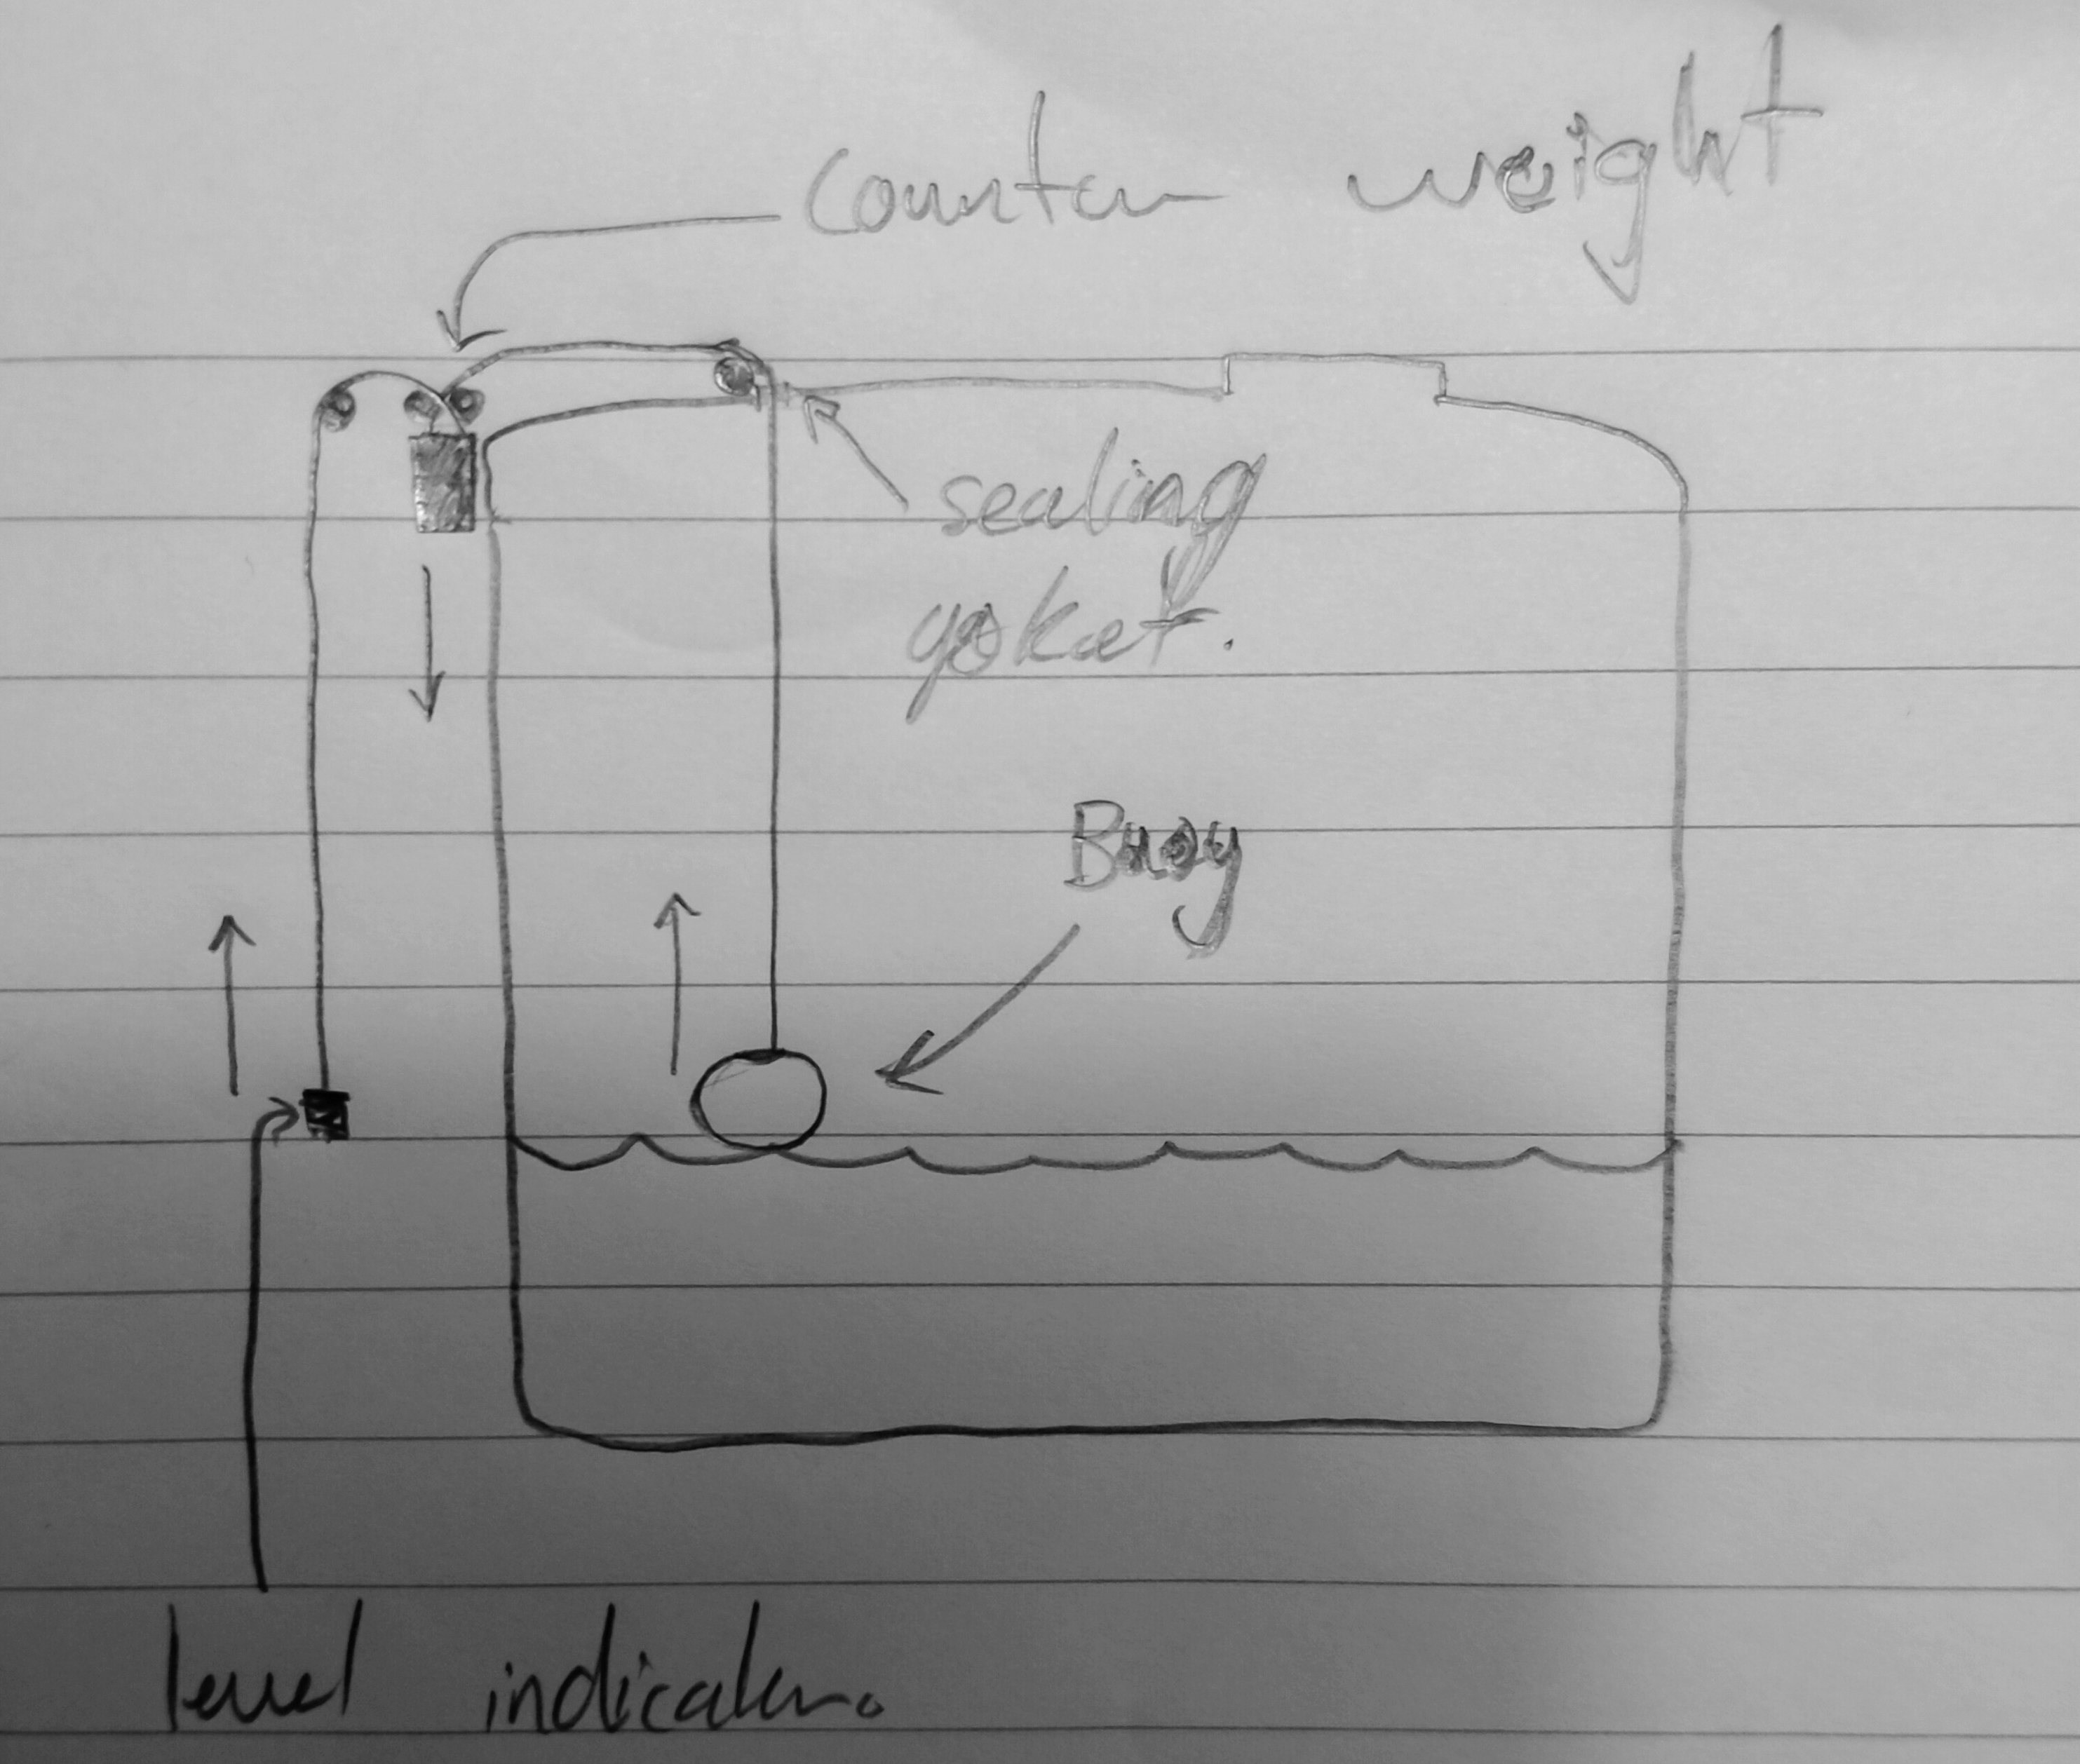
\includegraphics[width=0.75\textwidth]{mk1.jpg}
\end{center}
\begin{itemize}
        \item Simple construction, with electrical requirements
        \item Is a non-reverse indicator. If properly aligned the level indicator will align with the internal water level
        \item If buoy is sized correctly to the tanks overflow level, they should be no or minimal clipping of mini/max levels.
        \item Included materials are 4 pulleys, rope, a seal, buoy, level indicator (small stainless steel ball/etc), counter-weight (sand filled plastic container), and mounting hardware. Total material cost should be below \$100 and take a maximum of 2 hours to install.  
\end{itemize}
\subsection*{Mk II}
MK I succeeds in simplicity and durability, but does not offer much extra. Points that can be improved include: 
\begin{itemize}
        \item Quantifiable output, i.e. volume, days left of consumption.
        \item Remote monitoring and alerts
        \item software based extension and future support.
\end{itemize} 
Utilising the MB7369 ultrasonic water level sensor, which is IP-68 water resistant, has a 7.65 meter range, 1cm resolution and 200,000 rating hours of inter-servicing operating time, it can be mounted above the overflow line inside the tank and the cable feed and sealed through a drill hole (or using an existing inspection hole) and provide and can provide either an analog voltage reading, PWM or digital (RS232) signal to a compatible  micro-controller.

\textit{cost:} \$40.00

To drive the system, the ESP32 controller can be installed in a weather project box at the base of tank and powered via a DC PSU from the nearby main connection. The sensor has a low current draw of 3.4mA @ 3-5V5 so can be driven from the onboard V-reg.
This board provides low power Bluetooth, wifi, and a duel core processor with lower power functionality.

\textit{cost:} \$3-\$6

With this an external display can be driven either mounted at the box or remotely connect indoors (via BLE or wifi). It will display the current level in meters/volume and estimated remaining days calculated from usage.

\textit{cost:} \$15

All extra component cost under \$50 and time and development time estimated at 15-20hr.

The system provide the possible expansion via firmware updates (ESP32 allows this to be set up remotely) to a Mk III installation of a possible mobile app or website based monitoring 

\section*{Question 2}
$E=2.2{\times}10^{11}\;N/m^2,\; S_{max} = 5.5{\times}10^8\;N/m^2,\;G=2.2$

$x=8cm,\;t=0.15cm,\;w=2.5cm,\;R=150\Omega$
$$E=\frac{S}{\varepsilon} \Rightarrow \varepsilon =\frac{S}{E} = 2.5{\times}10^{-3}$$
$$\varepsilon = \frac{6xF}{wt^2E} \Rightarrow F = \frac{{\varepsilon}wt^2E}{6X} = 67.03N$$
$$G = \frac{{\Delta}R/R}{\varepsilon} \Rightarrow {\Delta}R = G{\varepsilon}R = 0.825\Omega$$
\section*{Question 3}
$$0.1\;arcmin = 0.001667^{\circ}$$
$$360/0.001667 = 215956.8 \Rightarrow \mathrm{round\;to\;} 215957$$
$$log_2(215957) = 17.72,\;\mathrm{ie\;\textbf{18bit}\;absolute\;encoder}$$
\section*{Question 4}
$\varepsilon_{emf} = -S{\Delta}T$

$$750{\mu}V = -S(70-10)\;\therefore\;-S=12.5{\mu}V/^{\circ}C$$
$$520{\mu}V = 12.5(t-10)$$
$$t = \frac{520}{12.5}+10 = 51.6^{\circ}C$$

With the rough estimate of sensitivity above of $12.5{\mu}V/^{\circ}C$, this closest resembles a type R, platinum-rhodium thermocouple, which have a nomnial sensitivity of around 9 at room temp. As opposed to a type K (chromel and alumel) of 41.
\section*{Question 5}
$$\varepsilon_{emf} = -S{\Delta}T$$
$$= 12.5(-35)=-437.5{\mu}V$$

\section*{Question 6}
\begin{enumerate}[label=\roman*)]
        \item Taking the pot as a voltage divider:
                $$V_{oc} = Vs\left(\frac{R_{p}x}{R_{p}x + R_{p}(1-x)}\right)$$

                With load resistance, $R_{out}$ becomes $R_px{\parallelsum}R_L$

                $$V_L = V_s\left( \frac{R_px{\parallelsum}R_L}{R_px{\parallelsum}R_L + P_px(1-x)} \right)$$
                $$= V_s\left( \frac{\frac{R_px{\cdot}R_L}{R_px+R_L}}{\frac{R_px{\cdot}R_L}{R_px+R_L} + R_px(1-x)} \right)$$
                $$=Vs\left( \frac{R_Lx}{R_L + R_px(1-x)} \right)$$
                $$=x{\cdot}Vs\left( \frac{1}{1 + {R_p}{R_L}x(1-x)} \right)$$
                Loading error is defined as: $N(x) = V_{oc} - V_L$ 
                $$N(x) = Vs\left( \frac{R_{p}x}{R_{p}x + R_{p}(1-x)} -  \frac{x}{1 + {R_p}{R_L}x(1-x)}\right)$$
        \item If $\frac{R_p}{R_L} << 1$ then the Loading error can be simplified to $V_s{\cdot}(x^2 - x^3){\cdot}\frac{R_p}{R_L}$

        Differentiate: $V_s{\cdot}\frac{R_p}{R_L}{\cdot}(2x - 3x^2)$

        $(2x - 3x^2)=0\;:\;x=2/3$

        $N(x)_{max} = (4/27)V_s{\cdot}\frac{R_p}{R_L} \therefore$ maximum error percentage is $N(x)_{max}/V_s {\times} 100 = 400/27{\cdot}\frac{R_p}{R_L} = 400/27 = 14.814815 \approx 15{\cdot}\frac{R_p}{R_L}$ 
        \item 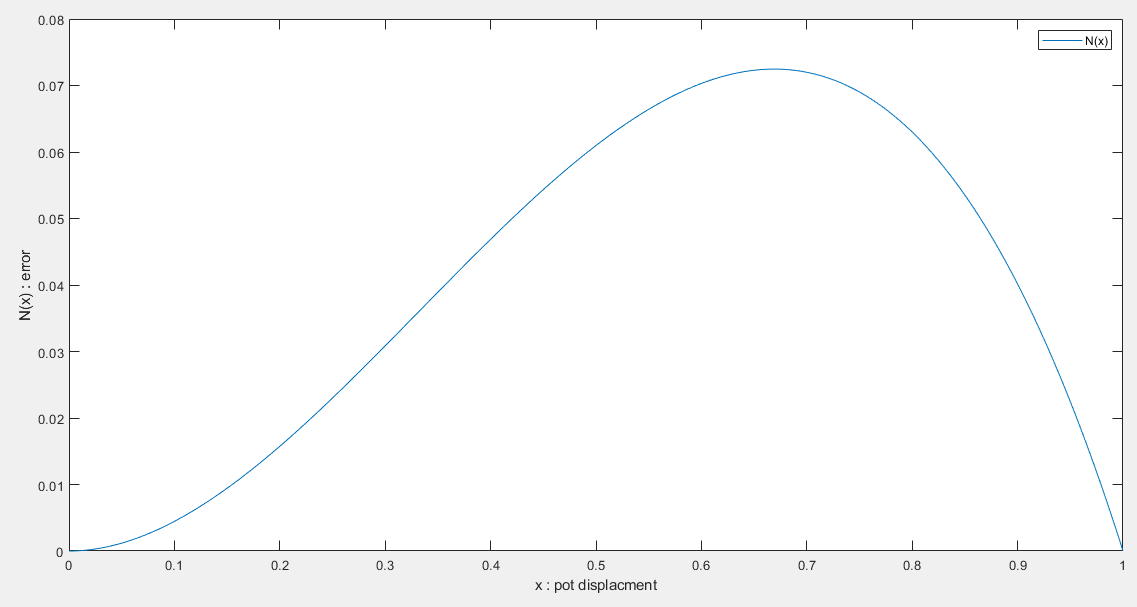
\includegraphics[width=0.7\textwidth]{error_plot.png}
        \item By knowing the points of maximum error and the characteristics of how the system approaches it, the transducer can be designed in such a way as to the operating region. 
        \item (a,b) Using max error will ensure it's under requirement across whole displacement, ie fore both, 0.2 and 0.67. 
        $$0.1 = 15(1k/R_L)$$
        $$R_L = 15k/0.1=150k$$
\end{enumerate}

\end{document}